\documentclass[twoside]{book}

% Packages required by doxygen
\usepackage{calc}
\usepackage{doxygen}
\usepackage{graphicx}
\usepackage[utf8]{inputenc}
\usepackage{makeidx}
\usepackage{multicol}
\usepackage{multirow}
\usepackage{textcomp}
\usepackage[table]{xcolor}

% Font selection
\usepackage[T1]{fontenc}
\usepackage{mathptmx}
\usepackage[scaled=.90]{helvet}
\usepackage{courier}
\usepackage{amssymb}
\usepackage{sectsty}
\renewcommand{\familydefault}{\sfdefault}
\allsectionsfont{%
  \fontseries{bc}\selectfont%
  \color{darkgray}%
}
\renewcommand{\DoxyLabelFont}{%
  \fontseries{bc}\selectfont%
  \color{darkgray}%
}

% Page & text layout
\usepackage{geometry}
\geometry{%
  a4paper,%
  top=2.5cm,%
  bottom=2.5cm,%
  left=2.5cm,%
  right=2.5cm%
}
\tolerance=750
\hfuzz=15pt
\hbadness=750
\setlength{\emergencystretch}{15pt}
\setlength{\parindent}{0cm}
\setlength{\parskip}{0.2cm}
\makeatletter
\renewcommand{\paragraph}{%
  \@startsection{paragraph}{4}{0ex}{-1.0ex}{1.0ex}{%
    \normalfont\normalsize\bfseries\SS@parafont%
  }%
}
\renewcommand{\subparagraph}{%
  \@startsection{subparagraph}{5}{0ex}{-1.0ex}{1.0ex}{%
    \normalfont\normalsize\bfseries\SS@subparafont%
  }%
}
\makeatother

% Headers & footers
\usepackage{fancyhdr}
\pagestyle{fancyplain}
\fancyhead[LE]{\fancyplain{}{\bfseries\thepage}}
\fancyhead[CE]{\fancyplain{}{}}
\fancyhead[RE]{\fancyplain{}{\bfseries\leftmark}}
\fancyhead[LO]{\fancyplain{}{\bfseries\rightmark}}
\fancyhead[CO]{\fancyplain{}{}}
\fancyhead[RO]{\fancyplain{}{\bfseries\thepage}}
\fancyfoot[LE]{\fancyplain{}{}}
\fancyfoot[CE]{\fancyplain{}{}}
\fancyfoot[RE]{\fancyplain{}{\bfseries\scriptsize Generated on Wed Apr 9 2014 13\-:01\-:42 for jaastool by Doxygen }}
\fancyfoot[LO]{\fancyplain{}{\bfseries\scriptsize Generated on Wed Apr 9 2014 13\-:01\-:42 for jaastool by Doxygen }}
\fancyfoot[CO]{\fancyplain{}{}}
\fancyfoot[RO]{\fancyplain{}{}}
\renewcommand{\footrulewidth}{0.4pt}
\renewcommand{\chaptermark}[1]{%
  \markboth{#1}{}%
}
\renewcommand{\sectionmark}[1]{%
  \markright{\thesection\ #1}%
}

% Indices & bibliography
\usepackage{natbib}
\usepackage[titles]{tocloft}
\setcounter{tocdepth}{3}
\setcounter{secnumdepth}{5}
\makeindex

% Custom commands
\newcommand{\clearemptydoublepage}{%
  \newpage{\pagestyle{empty}\cleardoublepage}%
}


%===== C O N T E N T S =====

\begin{document}

% Titlepage & ToC
\pagenumbering{roman}
\begin{titlepage}
\vspace*{7cm}
\begin{center}%
{\Large jaastool \\[1ex]\large 1.\-0-\/0 }\\
\vspace*{1cm}
{\large Generated by Doxygen 1.8.6}\\
\vspace*{0.5cm}
{\small Wed Apr 9 2014 13:01:42}\\
\end{center}
\end{titlepage}
\clearemptydoublepage
\tableofcontents
\clearemptydoublepage
\pagenumbering{arabic}

%--- Begin generated contents ---
\chapter{Java\-Doc A\-P\-I Markup for jaastool}
\label{index}\section*{jaastool }

J\+A\+A\+S Tools used to aid diagnosing opaque issues

B\+U\+I\+L\+D\+I\+N\+G

This is a standard Auto\+Tools build, so\+:

1) autoreconf -\/vfi

2) make install (or \char`\"{}make check\char`\"{} to include that plus run the tests)

3) make rpm (if so inclined)

java/jaastool.\+jar is the proper built jar file; convjars is where \char`\"{}convenience jars\char`\"{} are built if you're less concerned with license purity and more concerned with\+:

1) your tests are bogus. Let me test exactly what you tested; or

2) I need it working like yesterday. Holy crap please help me. Gimme something to download immediately to make the pain stop.

We've all been there. In both cases. grab convjars/jaastool.\+jar, it's not sanitary, but it works.

U\+S\+A\+G\+E

The only portion right is the \doxyref{Jaas\+No\+File.\+java}{p.}{JaasNoFile_8java_source} which nearly works as eloquently as implied. I use it for trying to see why a Kerberos client who shall remain nameless (V\+W-\/3) is not getting a clear result from the Kerberos server and/or not logging the full story. Also, said client is a great product, but in cases of customer doubt or dialect/terminology skew, this utility is a third-\/party to that argument. \begin{DoxyVerb}java -jar jaastool.jar -E
\end{DoxyVerb}


For more detail\+: \begin{DoxyVerb}java -jar jaastool.jar -EDv
\end{DoxyVerb}


Jaas\+Tool will then grab your username and domain as Principal and Realm, hit your L\+O\+G\+O\+N\+S\+E\+R\+V\+E\+R, and report the details verbosely. There will be a summary after it's all done.

o You'll be asked multiple times for your password. Don't worry, to avoid storing it, Jaas\+Tool re-\/asks.

o There will be a lot of java exception and Kerberos stuff. Don't worry, just wait for the summary at the end

o S\+E\+R\+I\+O\+U\+S\+L\+Y, do the password thing repeatedly until the summary. Details are all through that text.

The Sumary will tell you which principal@realm works at which servers (O\+K, which username@domain)

The code is hereby pasted to allow inspection and improve trust. Kerberos is used in secure environments. I get that, so I'm \char`\"{}opening the trenchcoat to show nothing stashed inside\char`\"{}.

Now go, get what you need, fix your pain! 
\chapter{R\-E\-A\-D\-M\-E}
\label{md_htdocs_README}
\input{md_htdocs_README}
\chapter{Hierarchical Index}
\section{Class Hierarchy}
This inheritance list is sorted roughly, but not completely, alphabetically\-:\begin{DoxyCompactList}
\item \contentsline{section}{Jaas\-No\-File}{\pageref{classorg_1_1smallfoot_1_1jaas_1_1JaasNoFile}}{}
\item Callback\-Handler\begin{DoxyCompactList}
\item \contentsline{section}{Jaas\-No\-File.\-Preregistered\-Password\-Callback}{\pageref{classorg_1_1smallfoot_1_1jaas_1_1JaasNoFile_1_1PreregisteredPasswordCallback}}{}
\end{DoxyCompactList}
\item Configuration\begin{DoxyCompactList}
\item \contentsline{section}{Jaas\-No\-File.\-No\-Conf\-File\-Configuration}{\pageref{classorg_1_1smallfoot_1_1jaas_1_1JaasNoFile_1_1NoConfFileConfiguration}}{}
\end{DoxyCompactList}
\end{DoxyCompactList}

\chapter{Data Structure Index}
\section{Data Structures}
Here are the data structures with brief descriptions\+:\begin{DoxyCompactList}
\item\contentsline{section}{{\bf Jaas\+No\+File} \\*Class and main function to iterate all combinations of given values to see which can successfully authenticate to a K\+R\+B service }{\pageref{classorg_1_1smallfoot_1_1jaas_1_1JaasNoFile}}{}
\item\contentsline{section}{{\bf Jaas\+No\+File.\+No\+Conf\+File\+Configuration} \\*Extends Configuration so that a krb5.\+conf is not needed; falls a bit short initially as bogus\+Config\+Block and libdefaults are both still needed }{\pageref{classorg_1_1smallfoot_1_1jaas_1_1JaasNoFile_1_1NoConfFileConfiguration}}{}
\item\contentsline{section}{{\bf Jaas\+No\+File.\+Preregistered\+Password\+Callback} \\*\doxyref{Preregistered\+Password\+Callback}{p.}{classorg_1_1smallfoot_1_1jaas_1_1JaasNoFile_1_1PreregisteredPasswordCallback} can be used later in the callback stack in place of the Text in order to type in the user's password for him/her }{\pageref{classorg_1_1smallfoot_1_1jaas_1_1JaasNoFile_1_1PreregisteredPasswordCallback}}{}
\end{DoxyCompactList}

\chapter{Data Structure Documentation}
\section{Jaas\+No\+File Class Reference}
\label{classorg_1_1smallfoot_1_1jaas_1_1JaasNoFile}\index{Jaas\+No\+File@{Jaas\+No\+File}}


Class and main function to iterate all combinations of given values to see which can successfully authenticate to a K\+R\+B service.  


\subsection*{Data Structures}
\begin{DoxyCompactItemize}
\item 
class {\bf No\+Conf\+File\+Configuration}
\begin{DoxyCompactList}\small\item\em extends Configuration so that a krb5.\+conf is not needed; falls a bit short initially as bogus\+Config\+Block and libdefaults are both still needed. \end{DoxyCompactList}\item 
class {\bf Preregistered\+Password\+Callback}
\begin{DoxyCompactList}\small\item\em \doxyref{Preregistered\+Password\+Callback}{p.}{classorg_1_1smallfoot_1_1jaas_1_1JaasNoFile_1_1PreregisteredPasswordCallback} can be used later in the callback stack in place of the Text in order to type in the user's password for him/her. \end{DoxyCompactList}\item 
class {\bfseries Text\+Confirm\+Action}
\end{DoxyCompactItemize}
\subsection*{Public Member Functions}
\begin{DoxyCompactItemize}
\item 
void {\bf usage} (String proc)\label{classorg_1_1smallfoot_1_1jaas_1_1JaasNoFile_a65d03ca5cd39f6905d34f7b0aab28f42}

\begin{DoxyCompactList}\small\item\em usage messages are useful to those of us with short memories as well (hey, I just need to add swap!) \end{DoxyCompactList}\end{DoxyCompactItemize}
\subsection*{Static Public Member Functions}
\begin{DoxyCompactItemize}
\item 
static void {\bf main} (String[$\,$] args)  throws Exception     
\begin{DoxyCompactList}\small\item\em Main function, nothing to see here... \end{DoxyCompactList}\end{DoxyCompactItemize}


\subsection{Detailed Description}
Class and main function to iterate all combinations of given values to see which can successfully authenticate to a K\+R\+B service. 

Definition at line 44 of file Jaas\+No\+File.\+java.



\subsection{Member Function Documentation}
\index{org\+::smallfoot\+::jaas\+::\+Jaas\+No\+File@{org\+::smallfoot\+::jaas\+::\+Jaas\+No\+File}!main@{main}}
\index{main@{main}!org\+::smallfoot\+::jaas\+::\+Jaas\+No\+File@{org\+::smallfoot\+::jaas\+::\+Jaas\+No\+File}}
\subsubsection[{main}]{\setlength{\rightskip}{0pt plus 5cm}static void main (
\begin{DoxyParamCaption}
\item[{String[$\,$]}]{args}
\end{DoxyParamCaption}
) throws Exception\hspace{0.3cm}{\ttfamily [inline]}, {\ttfamily [static]}}\label{classorg_1_1smallfoot_1_1jaas_1_1JaasNoFile_a8b260eecbaabcef8473fd87ada040682}


Main function, nothing to see here... 

this function uilds up a quick argument list with the intention if importing commandline arguments defining servers, domains/realms, usernames/principals, etc for use in hammering K\+D\+Cs later.


\begin{DoxyParams}{Parameters}
{\em args} & commandline arguments as described in the \doxyref{usage(\+String)}{p.}{classorg_1_1smallfoot_1_1jaas_1_1JaasNoFile_a65d03ca5cd39f6905d34f7b0aab28f42} function \\
\hline
\end{DoxyParams}
true == fudge the Realm into the environment. Part of the not-\/yet-\/eloquent part, I was trying to avoid having to do that. \+:(

true == fudge the K\+D\+C into the environment. Part of the not-\/yet-\/eloquent part, I was trying to avoid having to do that. \+:(

Definition at line 293 of file Jaas\+No\+File.\+java.



References Jaas\+No\+File.\+usage().



Here is the call graph for this function\+:
\nopagebreak
\begin{figure}[H]
\begin{center}
\leavevmode
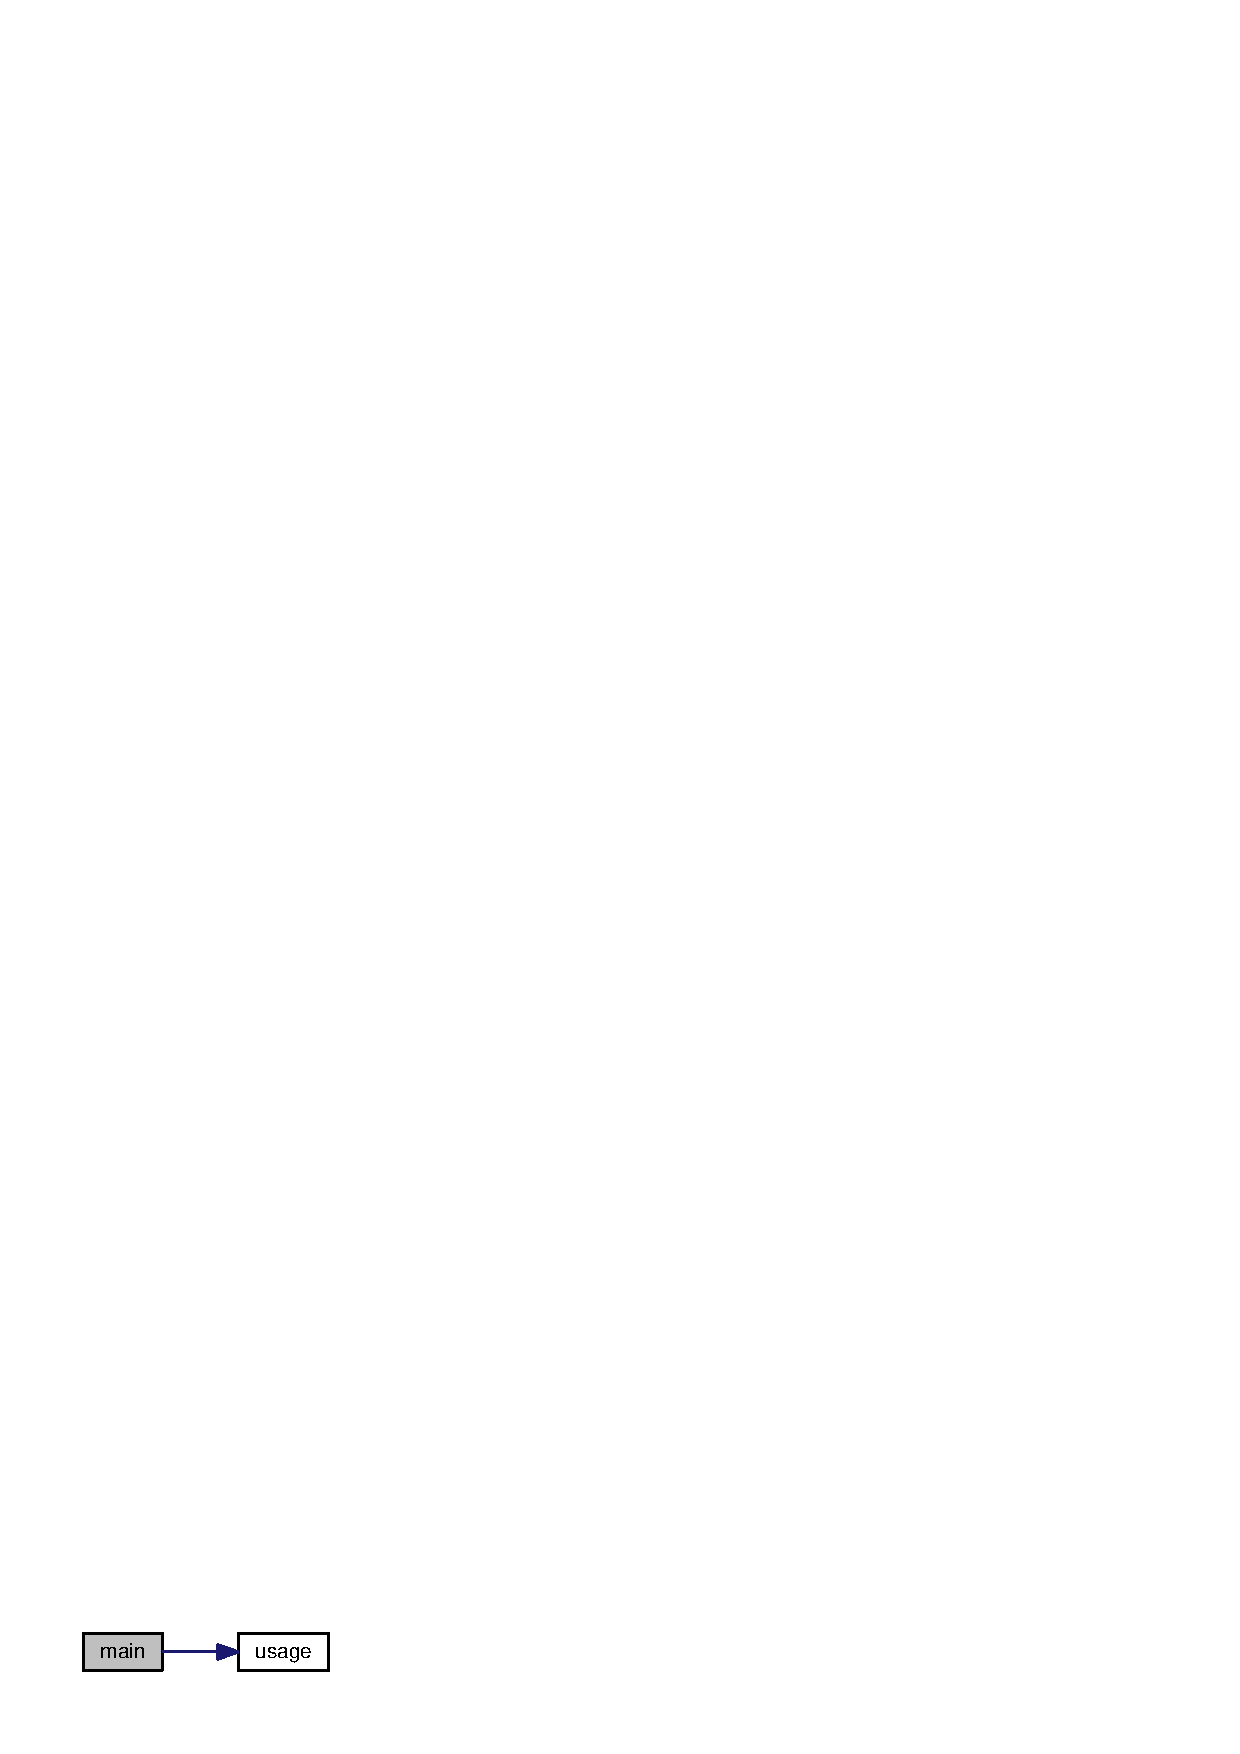
\includegraphics[width=162pt]{classorg_1_1smallfoot_1_1jaas_1_1JaasNoFile_a8b260eecbaabcef8473fd87ada040682_cgraph}
\end{center}
\end{figure}




The documentation for this class was generated from the following file\+:\begin{DoxyCompactItemize}
\item 
java/Jaas\+No\+File.\+java\end{DoxyCompactItemize}

\section{Jaas\-No\-File.\-No\-Conf\-File\-Configuration Class Reference}
\label{classorg_1_1smallfoot_1_1jaas_1_1JaasNoFile_1_1NoConfFileConfiguration}\index{Jaas\-No\-File.\-No\-Conf\-File\-Configuration@{Jaas\-No\-File.\-No\-Conf\-File\-Configuration}}


extends Configuration so that a krb5.\-conf is not needed; falls a bit short initially as bogus\-Config\-Block and libdefaults are both still needed.  




Inheritance diagram for Jaas\-No\-File.\-No\-Conf\-File\-Configuration\-:\nopagebreak
\begin{figure}[H]
\begin{center}
\leavevmode
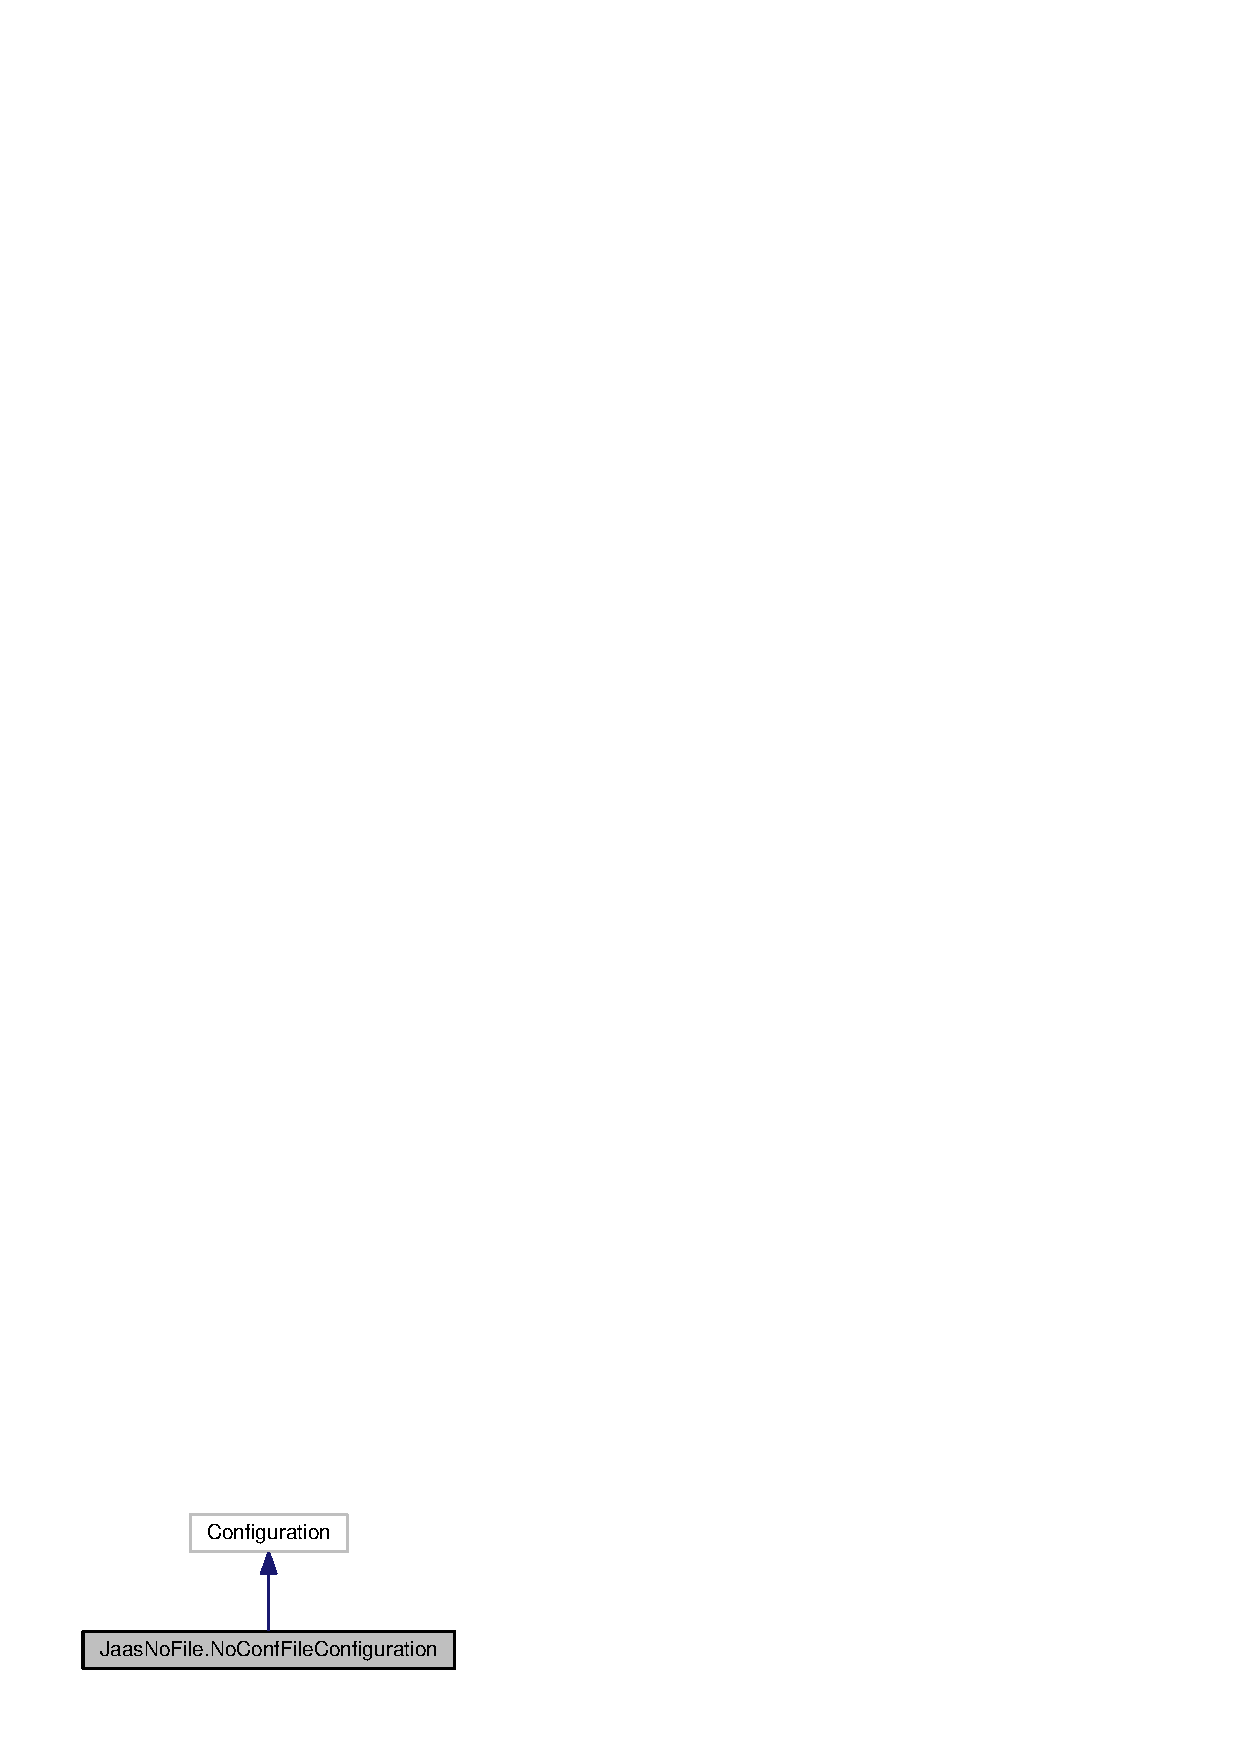
\includegraphics[width=222pt]{classorg_1_1smallfoot_1_1jaas_1_1JaasNoFile_1_1NoConfFileConfiguration__inherit__graph}
\end{center}
\end{figure}


Collaboration diagram for Jaas\-No\-File.\-No\-Conf\-File\-Configuration\-:\nopagebreak
\begin{figure}[H]
\begin{center}
\leavevmode
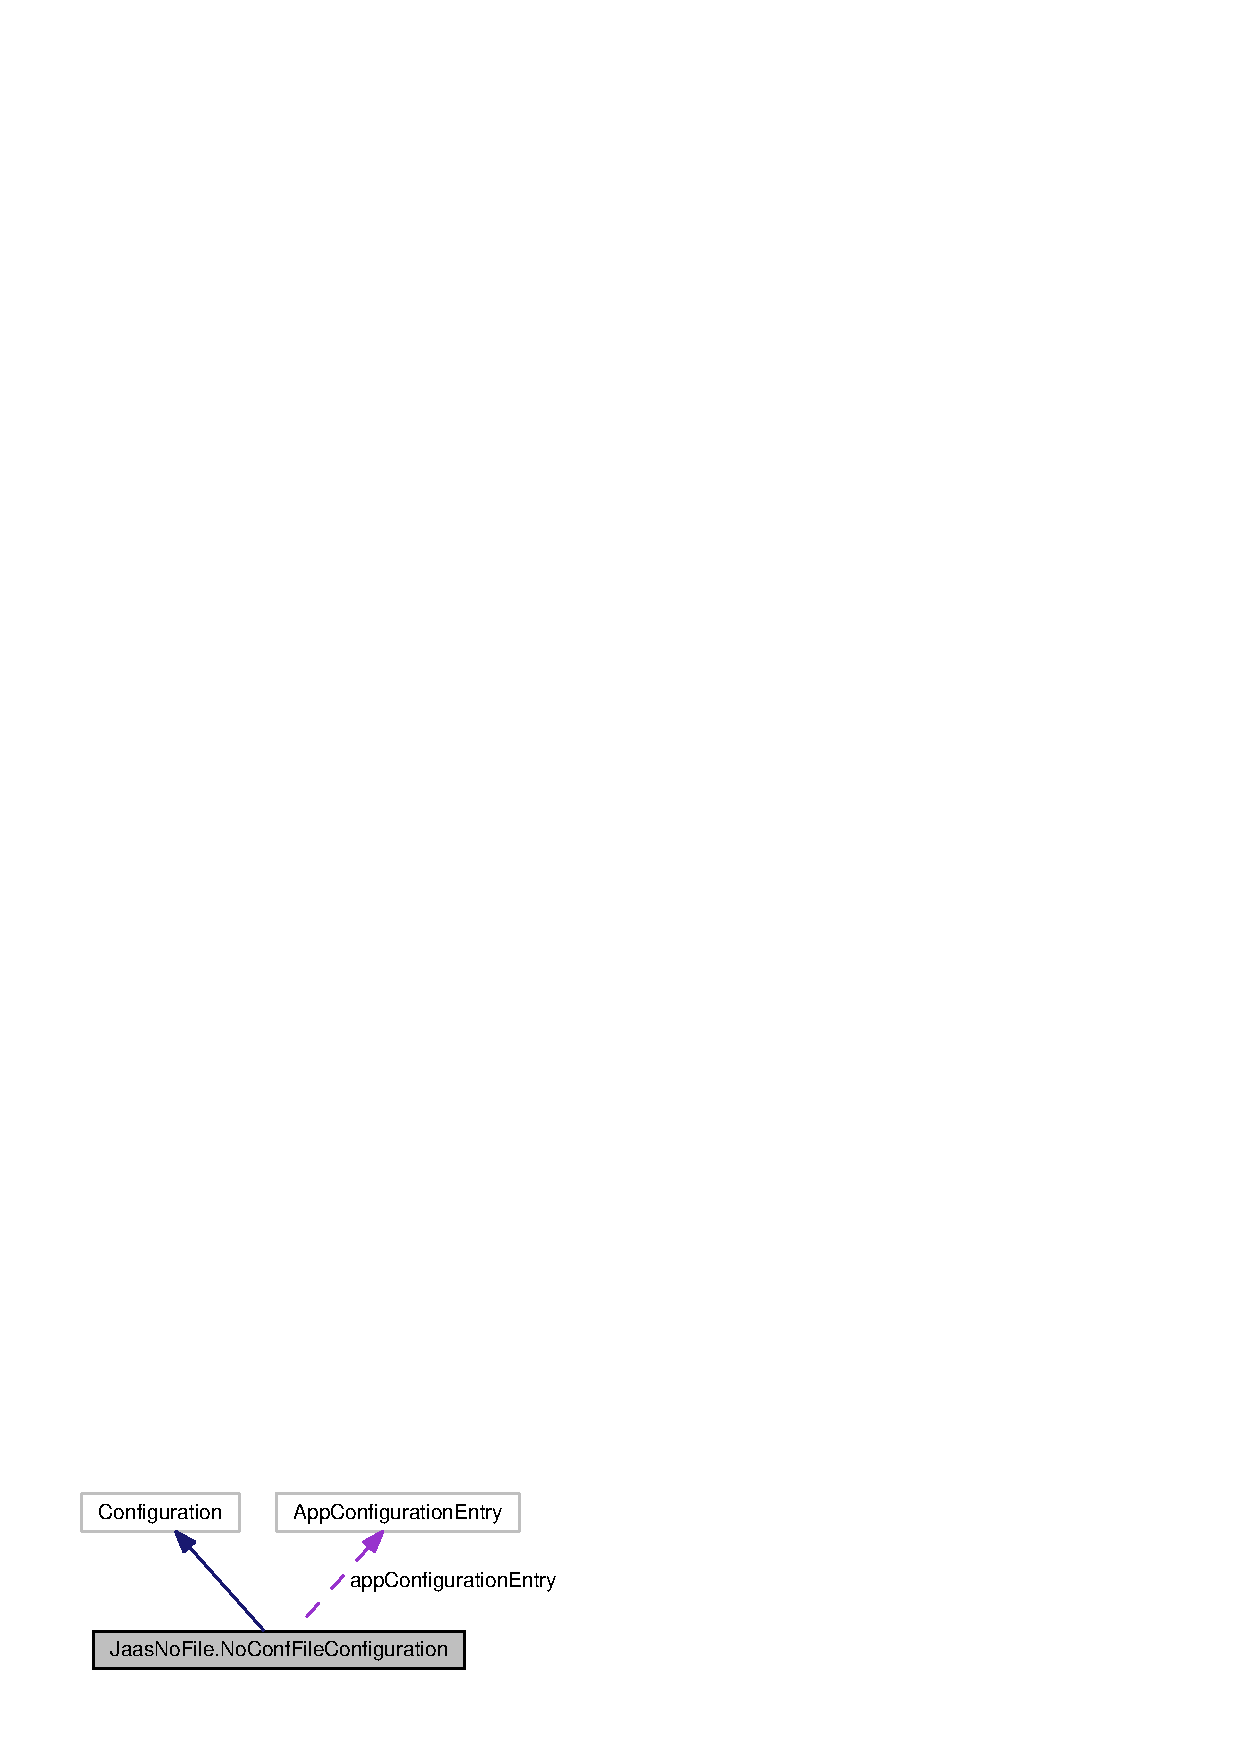
\includegraphics[width=271pt]{classorg_1_1smallfoot_1_1jaas_1_1JaasNoFile_1_1NoConfFileConfiguration__coll__graph}
\end{center}
\end{figure}
\subsection*{Public Member Functions}
\begin{DoxyCompactItemize}
\item 
App\-Configuration\-Entry[$\,$] {\bf get\-App\-Configuration\-Entry} (String x)
\begin{DoxyCompactList}\small\item\em offer out the configuration we have stored when the login process requests \end{DoxyCompactList}\item 
void {\bf refresh} ()
\begin{DoxyCompactList}\small\item\em Interface method for reloading the configuration, which is not done in this config. \end{DoxyCompactList}\end{DoxyCompactItemize}
\subsection*{Private Attributes}
\begin{DoxyCompactItemize}
\item 
App\-Configuration\-Entry {\bf app\-Configuration\-Entry}\label{classorg_1_1smallfoot_1_1jaas_1_1JaasNoFile_1_1NoConfFileConfiguration_a1641ae97493d812092dc82538dfeb1d1}

\begin{DoxyCompactList}\small\item\em the section of a virtual config file generated using the constructor No\-Conf\-File\-Configuration(\-String,\-String,\-String,\-String,boolean) \end{DoxyCompactList}\end{DoxyCompactItemize}


\subsection{Detailed Description}
extends Configuration so that a krb5.\-conf is not needed; falls a bit short initially as bogus\-Config\-Block and libdefaults are both still needed. 

This class mimicks the sections of a config file, if it existed, simulating sections of config information. Access is controlled through the \doxyref{get\-App\-Configuration\-Entry()}{p.}{classorg_1_1smallfoot_1_1jaas_1_1JaasNoFile_1_1NoConfFileConfiguration_a7b64232f7d996279c40eb859a017c11b} function, which metes out the included app\-Configuration\-Entry or not based on a section value. 

Definition at line 53 of file Jaas\-No\-File.\-java.



\subsection{Member Function Documentation}
\index{org\-::smallfoot\-::jaas\-::\-Jaas\-No\-File\-::\-No\-Conf\-File\-Configuration@{org\-::smallfoot\-::jaas\-::\-Jaas\-No\-File\-::\-No\-Conf\-File\-Configuration}!get\-App\-Configuration\-Entry@{get\-App\-Configuration\-Entry}}
\index{get\-App\-Configuration\-Entry@{get\-App\-Configuration\-Entry}!org::smallfoot::jaas::JaasNoFile::NoConfFileConfiguration@{org\-::smallfoot\-::jaas\-::\-Jaas\-No\-File\-::\-No\-Conf\-File\-Configuration}}
\subsubsection[{get\-App\-Configuration\-Entry}]{\setlength{\rightskip}{0pt plus 5cm}App\-Configuration\-Entry [$\,$] get\-App\-Configuration\-Entry (
\begin{DoxyParamCaption}
\item[{String}]{x}
\end{DoxyParamCaption}
)\hspace{0.3cm}{\ttfamily [inline]}}\label{classorg_1_1smallfoot_1_1jaas_1_1JaasNoFile_1_1NoConfFileConfiguration_a7b64232f7d996279c40eb859a017c11b}


offer out the configuration we have stored when the login process requests 


\begin{DoxyParams}{Parameters}
{\em x} & name of the section being requested\-: \char`\"{}client\char`\"{} causes the generated seciton to be returned, an empty section otherwise \\
\hline
\end{DoxyParams}
\begin{DoxyReturn}{Returns}
an App\-Configuration\-Entry that is either blank, or a client config block similar to \char`\"{}[client]\char`\"{} section in krb5.\-conf
\end{DoxyReturn}
\begin{DoxySeeAlso}{See Also}
{\tt http\-://web.\-mit.\-edu/kerberos/krb5-\/1.\-5/krb5-\/1.\-5/doc/krb5-\/admin/krb5.\-conf.\-html} 
\end{DoxySeeAlso}


Definition at line 122 of file Jaas\-No\-File.\-java.



References Jaas\-No\-File.\-No\-Conf\-File\-Configuration.\-app\-Configuration\-Entry.

\index{org\-::smallfoot\-::jaas\-::\-Jaas\-No\-File\-::\-No\-Conf\-File\-Configuration@{org\-::smallfoot\-::jaas\-::\-Jaas\-No\-File\-::\-No\-Conf\-File\-Configuration}!refresh@{refresh}}
\index{refresh@{refresh}!org::smallfoot::jaas::JaasNoFile::NoConfFileConfiguration@{org\-::smallfoot\-::jaas\-::\-Jaas\-No\-File\-::\-No\-Conf\-File\-Configuration}}
\subsubsection[{refresh}]{\setlength{\rightskip}{0pt plus 5cm}void refresh (
\begin{DoxyParamCaption}
{}
\end{DoxyParamCaption}
)\hspace{0.3cm}{\ttfamily [inline]}}\label{classorg_1_1smallfoot_1_1jaas_1_1JaasNoFile_1_1NoConfFileConfiguration_a5f2e190b8261a98c97c2ea4e86670d54}


Interface method for reloading the configuration, which is not done in this config. 

I'm trying to provide this to avoid \char`\"{}reloading\char`\"{} a config that is virtual and breaking the minds of the poor machines who want to reload from disk or such. ..because disk is, like, so last week. 

Definition at line 136 of file Jaas\-No\-File.\-java.



The documentation for this class was generated from the following file\-:\begin{DoxyCompactItemize}
\item 
java/Jaas\-No\-File.\-java\end{DoxyCompactItemize}

\section{Jaas\-No\-File.\-Preregistered\-Password\-Callback Class Reference}
\label{classorg_1_1smallfoot_1_1jaas_1_1JaasNoFile_1_1PreregisteredPasswordCallback}\index{Jaas\-No\-File.\-Preregistered\-Password\-Callback@{Jaas\-No\-File.\-Preregistered\-Password\-Callback}}


\doxyref{Preregistered\-Password\-Callback}{p.}{classorg_1_1smallfoot_1_1jaas_1_1JaasNoFile_1_1PreregisteredPasswordCallback} can be used later in the callback stack in place of the Text in order to type in the user's password for him/her.  




Inheritance diagram for Jaas\-No\-File.\-Preregistered\-Password\-Callback\-:\nopagebreak
\begin{figure}[H]
\begin{center}
\leavevmode
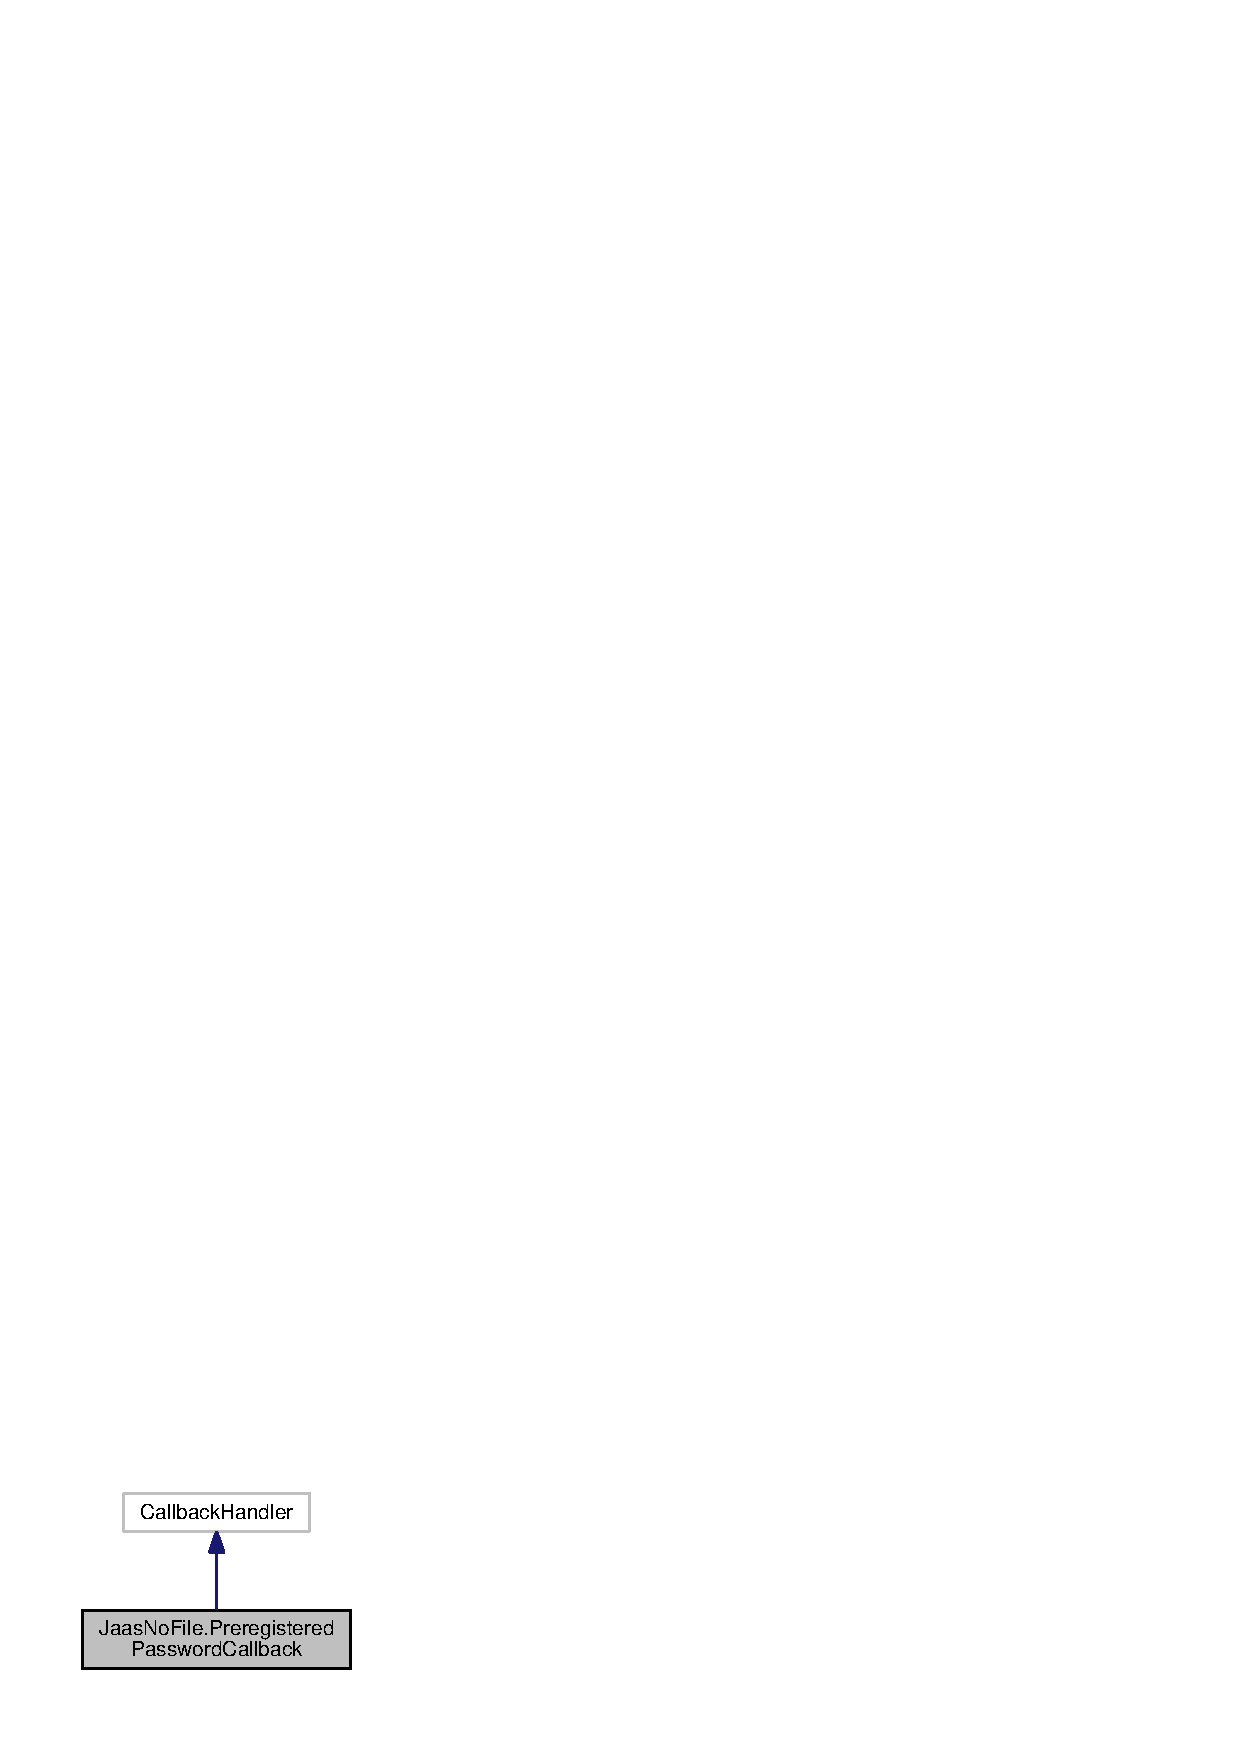
\includegraphics[width=172pt]{classorg_1_1smallfoot_1_1jaas_1_1JaasNoFile_1_1PreregisteredPasswordCallback__inherit__graph}
\end{center}
\end{figure}


Collaboration diagram for Jaas\-No\-File.\-Preregistered\-Password\-Callback\-:\nopagebreak
\begin{figure}[H]
\begin{center}
\leavevmode
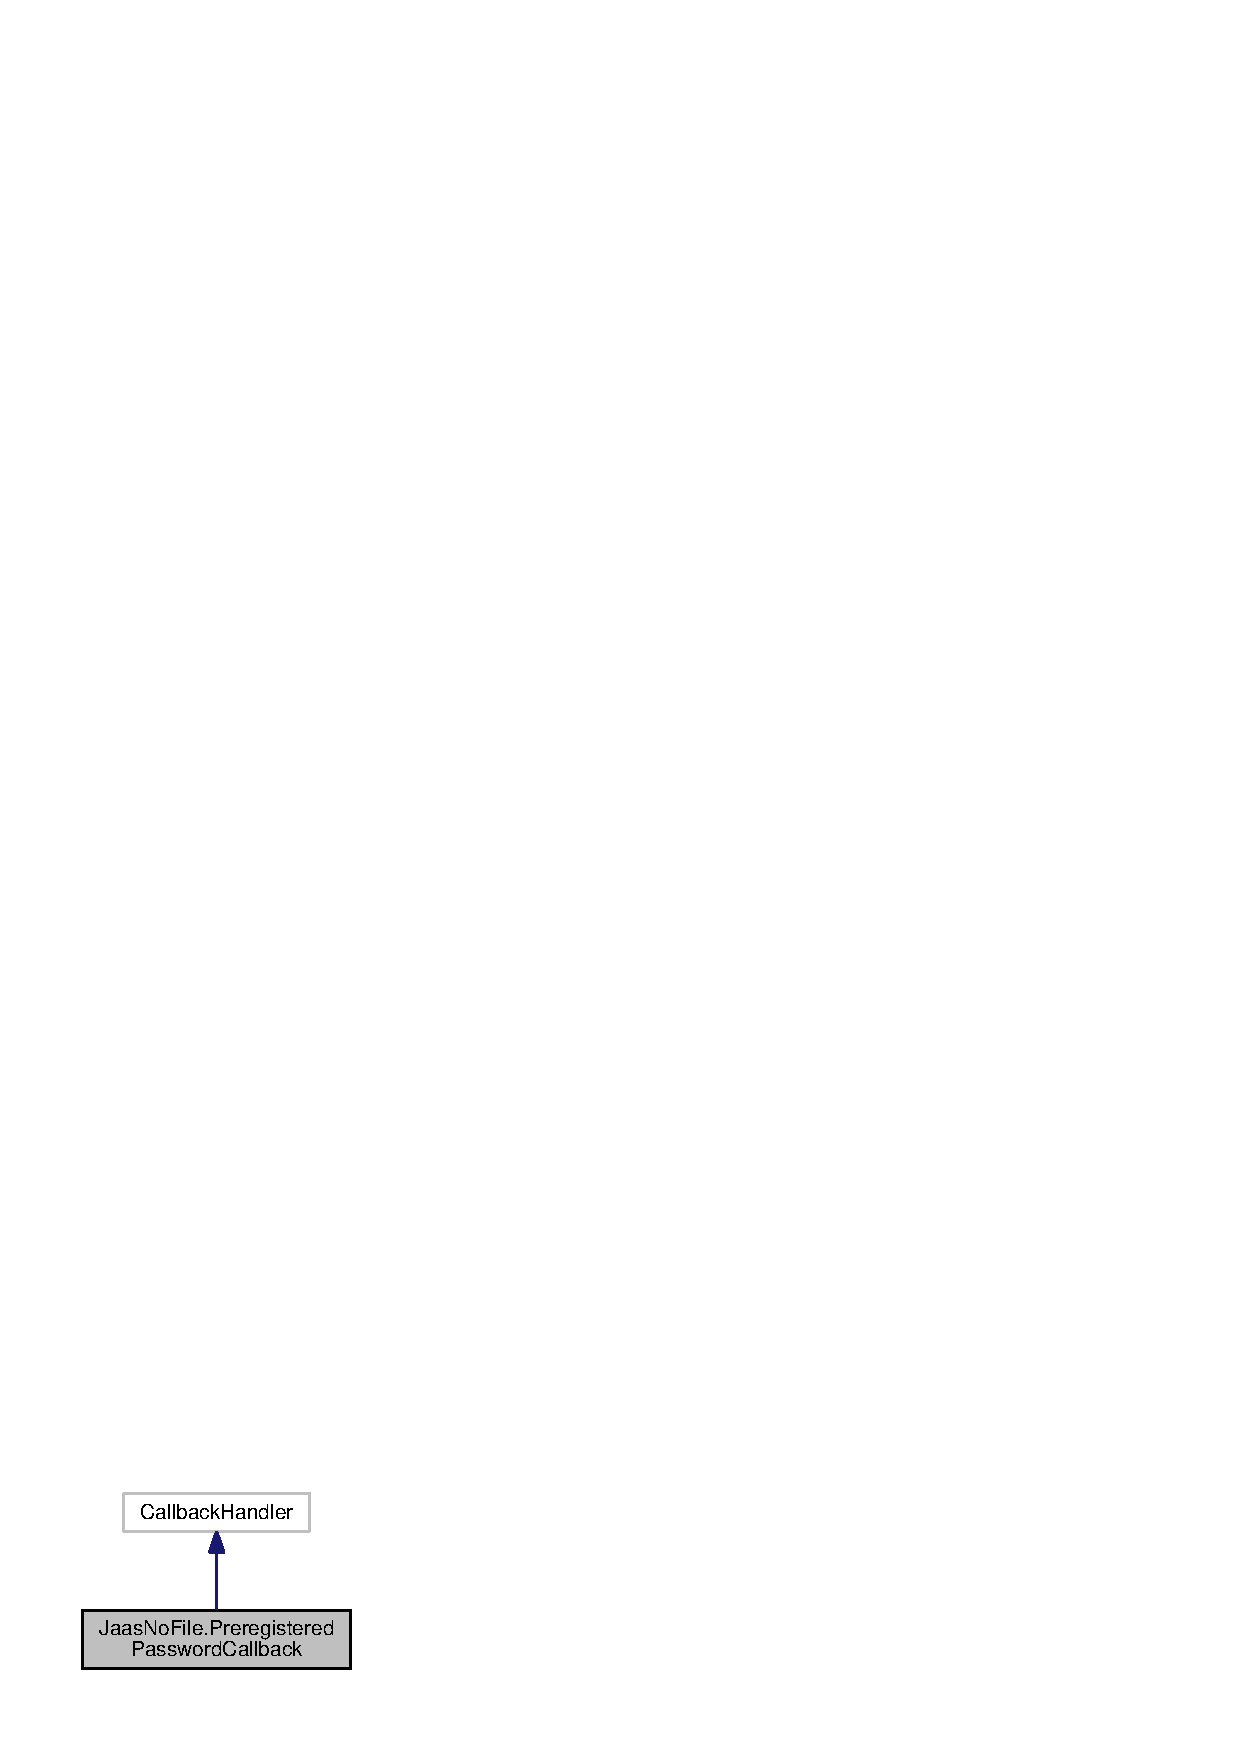
\includegraphics[width=172pt]{classorg_1_1smallfoot_1_1jaas_1_1JaasNoFile_1_1PreregisteredPasswordCallback__coll__graph}
\end{center}
\end{figure}
\subsection*{Public Member Functions}
\begin{DoxyCompactItemize}
\item 
{\bf Preregistered\-Password\-Callback} (String {\bf username}, String {\bf password})
\begin{DoxyCompactList}\small\item\em create the local authentication record for use later in \doxyref{handle(\-Callback[$\,$])}{p.}{classorg_1_1smallfoot_1_1jaas_1_1JaasNoFile_1_1PreregisteredPasswordCallback_a21117aca6aecc3046d9c31d604404e63} \end{DoxyCompactList}\item 
void {\bf handle} (Callback[$\,$] callbacks)  throws Unsupported\-Callback\-Exception   
\begin{DoxyCompactList}\small\item\em Attempts to log in using the username and password supplied during constructor. \end{DoxyCompactList}\end{DoxyCompactItemize}
\subsection*{Private Attributes}
\begin{DoxyCompactItemize}
\item 
String {\bf password}\label{classorg_1_1smallfoot_1_1jaas_1_1JaasNoFile_1_1PreregisteredPasswordCallback_acbd76b816d055b7a642c219fd9751020}

\begin{DoxyCompactList}\small\item\em password (plaintext) to use during authentication in \doxyref{handle(\-Callback[$\,$])}{p.}{classorg_1_1smallfoot_1_1jaas_1_1JaasNoFile_1_1PreregisteredPasswordCallback_a21117aca6aecc3046d9c31d604404e63} \end{DoxyCompactList}\item 
String {\bf username}\label{classorg_1_1smallfoot_1_1jaas_1_1JaasNoFile_1_1PreregisteredPasswordCallback_ae91c86c4d1584286de9492f51957ac23}

\begin{DoxyCompactList}\small\item\em principal or username to use during authentication in \doxyref{handle(\-Callback[$\,$])}{p.}{classorg_1_1smallfoot_1_1jaas_1_1JaasNoFile_1_1PreregisteredPasswordCallback_a21117aca6aecc3046d9c31d604404e63} \end{DoxyCompactList}\end{DoxyCompactItemize}


\subsection{Detailed Description}
\doxyref{Preregistered\-Password\-Callback}{p.}{classorg_1_1smallfoot_1_1jaas_1_1JaasNoFile_1_1PreregisteredPasswordCallback} can be used later in the callback stack in place of the Text in order to type in the user's password for him/her. 

This lets a host of possibilities be tried non-\/interactively 

Definition at line 246 of file Jaas\-No\-File.\-java.



\subsection{Constructor \& Destructor Documentation}
\index{org\-::smallfoot\-::jaas\-::\-Jaas\-No\-File\-::\-Preregistered\-Password\-Callback@{org\-::smallfoot\-::jaas\-::\-Jaas\-No\-File\-::\-Preregistered\-Password\-Callback}!Preregistered\-Password\-Callback@{Preregistered\-Password\-Callback}}
\index{Preregistered\-Password\-Callback@{Preregistered\-Password\-Callback}!org::smallfoot::jaas::JaasNoFile::PreregisteredPasswordCallback@{org\-::smallfoot\-::jaas\-::\-Jaas\-No\-File\-::\-Preregistered\-Password\-Callback}}
\subsubsection[{Preregistered\-Password\-Callback}]{\setlength{\rightskip}{0pt plus 5cm}{\bf Preregistered\-Password\-Callback} (
\begin{DoxyParamCaption}
\item[{String}]{username, }
\item[{String}]{password}
\end{DoxyParamCaption}
)\hspace{0.3cm}{\ttfamily [inline]}}\label{classorg_1_1smallfoot_1_1jaas_1_1JaasNoFile_1_1PreregisteredPasswordCallback_af03808b7e0079e3e73d4850951f7a5e9}


create the local authentication record for use later in \doxyref{handle(\-Callback[$\,$])}{p.}{classorg_1_1smallfoot_1_1jaas_1_1JaasNoFile_1_1PreregisteredPasswordCallback_a21117aca6aecc3046d9c31d604404e63} 


\begin{DoxyParams}{Parameters}
{\em username} & principal or username to use \\
\hline
{\em password} & plaintext password to use \\
\hline
\end{DoxyParams}


Definition at line 257 of file Jaas\-No\-File.\-java.



References Jaas\-No\-File.\-Preregistered\-Password\-Callback.\-password, and Jaas\-No\-File.\-Preregistered\-Password\-Callback.\-username.



\subsection{Member Function Documentation}
\index{org\-::smallfoot\-::jaas\-::\-Jaas\-No\-File\-::\-Preregistered\-Password\-Callback@{org\-::smallfoot\-::jaas\-::\-Jaas\-No\-File\-::\-Preregistered\-Password\-Callback}!handle@{handle}}
\index{handle@{handle}!org::smallfoot::jaas::JaasNoFile::PreregisteredPasswordCallback@{org\-::smallfoot\-::jaas\-::\-Jaas\-No\-File\-::\-Preregistered\-Password\-Callback}}
\subsubsection[{handle}]{\setlength{\rightskip}{0pt plus 5cm}void handle (
\begin{DoxyParamCaption}
\item[{Callback[$\,$]}]{callbacks}
\end{DoxyParamCaption}
) throws Unsupported\-Callback\-Exception\hspace{0.3cm}{\ttfamily [inline]}}\label{classorg_1_1smallfoot_1_1jaas_1_1JaasNoFile_1_1PreregisteredPasswordCallback_a21117aca6aecc3046d9c31d604404e63}


Attempts to log in using the username and password supplied during constructor. 


\begin{DoxyParams}{Parameters}
{\em callbacks} & list of callback structures which require filling in with the pre-\/defined data \\
\hline
\end{DoxyParams}


Definition at line 268 of file Jaas\-No\-File.\-java.



The documentation for this class was generated from the following file\-:\begin{DoxyCompactItemize}
\item 
java/Jaas\-No\-File.\-java\end{DoxyCompactItemize}

%--- End generated contents ---

% Index
\newpage
\phantomsection
\addcontentsline{toc}{chapter}{Index}
\printindex

\end{document}
